\chapter{Appendix A - Notes on Project Selection and Prior Work}

Without a background in air quality before this year, a large portion of the thesis was getting up to speed with the community, learning where the issues are, and trying to understand where advances might be made.  The thesis you've read is drastically different than the thesis I proposed ten months ago.

The first path we started down was to design and build some basic prototypes for chambering air samples.  The concept was to introduce these devices in high wind environments (like on a car or bicycle), and sample the air by sealing it in a chamber and tagging it with GPS coordinates.  Once a reading from an electrochemical gas sensor or another type of sensor had reached steady-state, we would evacuate the chamber and resample.  This inter-sample settling time could be learned and/or evaluated in real-time for varying conditions.

Below are mockups of two prototypes we 3D printed and prototyped for AlphaSense electrochemical gas sensors.  One is modeled after their calibration accessory (with a motorized paddle that seals the chamber when closed), and one is modeled after a revolver (with a spinning opening).  Another prototype we discussed was a cyringe style design, which has benefits for controlling chamber pressurization.
 
\begin{figure}[htb]
 	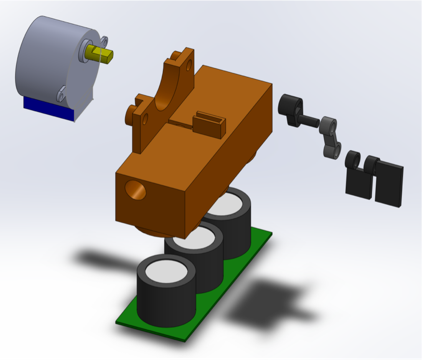
\includegraphics[width=\textwidth/2]{visuals/prevwork1a}    
 	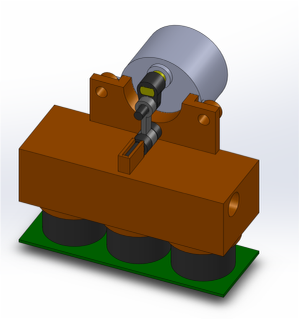
\includegraphics[width=\textwidth/2]{visuals/prevwork1b}            
 	 \caption{Original Concept \#1}
  	\label{fig:prevwork1a}
\end{figure}


The first of these was physically prototyped using the AlphaSense AFE board, an Arduino, and a ReadBearLabs Bluetooth LE Arduino Shield.  It was connected to a smartphone where it reported values, and could be commanded to open or close the chamber from the phone.

\begin{figure}[htb]
 	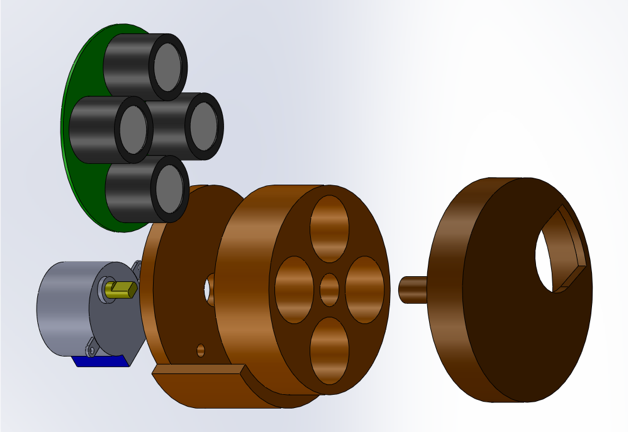
\includegraphics[width=\textwidth/2]{visuals/prevwork2a}    
 	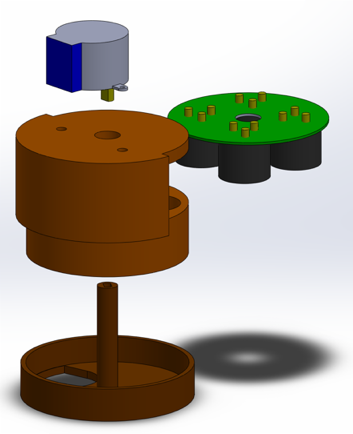
\includegraphics[width=\textwidth/2]{visuals/prevwork2b}            
 	 \caption{Original Concept \#2}
  	\label{fig:prevwork1a}
\end{figure}


After several more discussions, I decided to change directions and focus on some of the problems that I perceived to have more direct impact.  In general, there seems to be trust of the AlphaSense sensors in a mobile context, without discrete air sampling (regardless of whether this is a correct assumption-- to my knowledge, it has not yet been tested appropriately).  The needs of the air quality community seem to be at an earlier stage-- how to share data, how to characterize consumer devices, and how to understand consumer sensor quality.  It seemed to be a waste of time to build another consumer device in a crowded space, when there are no standard mechanisms to verify its quality or spread its impact in the air quality community.  Additionally, there is skepticism towards mobile-first sensing.  There are still issues facing affordable \texit{stationary} sensing, and no rigorous precedent on which to validate truly mobile solutions.

It is my hope that within a few years, the leaders in the air quality community will be positioned to make strong claims about whether new devices (like the one proposed above) actually work.  I hope this work may help form the foundation for which those claims can be made.  While the goal is mobile, personal sensing, the principles herein apply equally strongly to affordable, dense, heterogeneous, sensor systems, which certainly will feature prominently in the future of air quality measurement. 

\clearpage
\newpage
